\section{Approach}


The multi-turn response selection tasks represent each dialogue as a triple $T=\langle C, R, L\rangle$, where $C=\{t_1, t_2,...,t_n\}$ represents the history turns. $R$ is a candidate response and $L$ is the $0/1$ label indicating whether $R$ is the correct response or a negative candidate. To incorporate the dependency information between the history turns, we design a straight-forward algorithm to extract the dialogue history $C$ into dialogues threads $\langle C_1, C_2, ..., C_M\rangle$ based on the predicted dependencies, along with an elaborately designed model to find the function $f(C_1, C_2, ..., C_M, R)$, which measures the matching score of each $(C, R)$ pair. Both the extraction algorithm and the model will be explained as follows.% in this section.

\subsection{Dialogue Extraction Algorithm}
\label{sec:DSA}
Since it's impossible for the large pre-trained language models to take all of the dialogue history turns as the input under the computational power nowadays, these models usually set a truncate window and only consider the top-k most recent turns or tokens. However, several dialogue threads may exist concurrently in two-party~\cite{DuPX17} or multi-party dialogues~\cite{TanWGWPGCY19}. Such coarse-grained truncating operation may not only bring in redundant turns from 
other dialogue threads, but also exclude the expected turns given earlier 
in the current dialogue thread, hurting the representation capability of pre-trained language models. Extracting the whole history into self-contained dialogue threads can help preserve more relevant turns and avoid the negative effects of encoding irrelevant turns by a single language model.




Motivated by the above, we aim to analyze the discourse structures in dialogue history at first. We utilize the discourse dependency parsing model for dialogues proposed by Shi and Huang~\shortcite{ShiH19}. It is a deep sequential model that achieves the state-of-the-art performance on the STAC corpus.
Instead of predicting the predefined relation types between Elementary Discourse Units(EDUs), we borrow the proposed model in this work to find if there exist dependency relations between utterances in the given dialogue history.
The model scans through the dialogue history and predicts the most likely parent turn for each turn. 
It finally constructs a dependency tree for each dialogue history with a confidence score 
on each edge.


\begin{algorithm}
	\scriptsize
	\SetAlgoNoLine 
	\SetKwInOut{Input}{\textbf{Input}}
	\SetKwInOut{Output}{\textbf{Output}} 
	
	\Input
	{
		The dependency tree $T$ with confidence scores on each edge $e_{ji}=(t_i, t_j, P_{ji})$, where $i.j=1, 2, ..., n$ and $j>i$;\\
		The threshold for the confidence score $P$.
	}
	\Output{
		The threads $C'=\langle C_1, C_2, ..., C_M\rangle$, and each is made up of a sequence of turns.
	}
	\BlankLine
	
	\For {$e_{ji}$ in $T$}{
		\If{$P_{ji}<P$}{delete $e_{ji}$ from $T$}
	}
	The forest $T' = T$\\
	The set of threads $C'=\emptyset$\\
	\For{each leaf node in $T'$ }{
		$C_{tmp} =$ all the node from the leaf node to the corresponding root.\\
		$C'=C'\cup C_{tmp}$
	}
	Rank the threads in $C'$ based on the index of the leaf node in descending order.
	
	\caption{The Dialogue Extraction Algorithm\label{alg:A}}
	\label{alg:DSA}
\end{algorithm}


Then, the dialogue extraction algorithm is designed to extract original long history into dialogue threads according to dependency tree $T$ and confidence scores. The algorithm is 
depicted in \algoref{alg:A}. $e_{ji}$ is a directed edge with head $t_i$ and tail $t_j$, 
indicating that turn $j$ is a reply of turn $i$ with probability $P_{ji}$.
The threshold $P$ is a hyper-parameter. It is noteworthy that we still follow the intuition 
that the turns closer to the responses are more likely to be useful than others. 
As a result, the threads are returned in ascending order according to the distance between 
the last turns in each thread and the response. 
An illustration of the algorithm is shown in Figure \ref{fig:algorithm}. The 7-turn dialogue history is extracted into three threads.
\begin{figure}
	\centering
	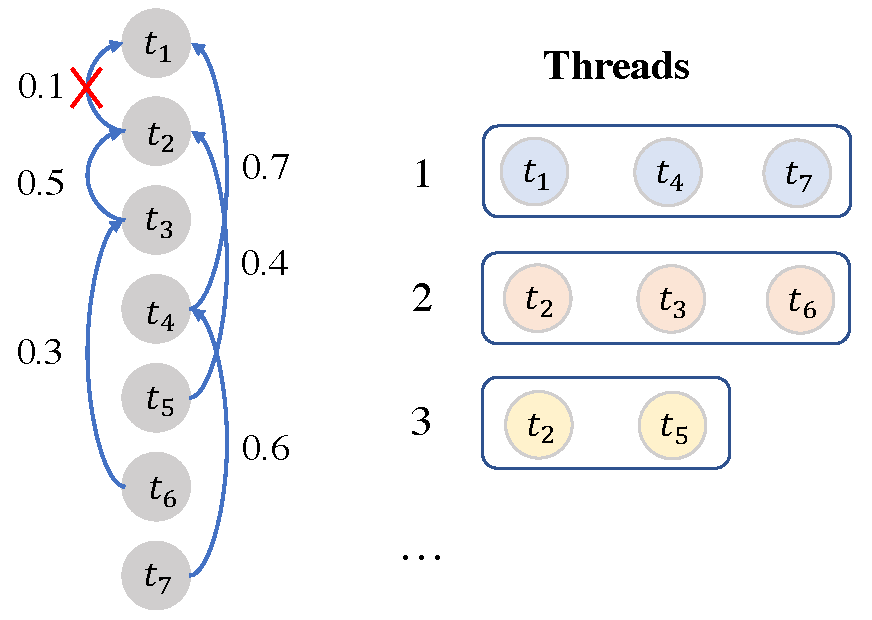
\includegraphics[scale=0.40]{pic/algorithm.pdf}
	\caption{An example of the algorithm when the threshold $P=0.2$. The figures are the confidence scores of corresponding predicted dependency relations.}
	\label{fig:algorithm}
\end{figure}

\subsection{Thread-based Encoder Model}
\label{sec:tem}
In the work from Humeau et al.~\shortcite{humeau2019poly}, they use a pre-trained language model as the context encoder and generate the embedding for dialogue history. Inspired by this work, we also utilize pre-trained language models to encode natural texts into meaningful representations.

Given the extracted self-contained dialogue threads $\langle C_1, C_2, ..., C_M \rangle$, we utilize a pre-trained language model to encode the content of each dialogue thread in parallel and another pre-trained language model to encode the candidate respectively. 
If the candidate representation matches well with one or more thread representations, 
that candidate is probably the correct response. 

The architecture of our model \textbf{Thread-Encoder} (shown in \figref{fig:model1}) can be divided into two layers: Encoding Layer and Matching Layer.

\subsubsection{Encoding Layer}
We use the pre-trained language model released by Humeau et al.~\shortcite{humeau2019poly}. This large pre-trained Transformer model has the same architecture as BERT-base \cite{DevlinCLT19}. It has 12 layers, 12 attention heads and 768 hidden size. Different from the original one trained on BooksCorpus and Wikipedia, the new language model is further trained on Reddit~\cite{abs-1904-06472}, a large dialogue dataset with around 727M context-response pairs. The pretraining tasks include masked language model and next utterance prediction~\footnote{``Utterance'' and ``turn'' are 
interchangeable in this paper.}. Finally, the pre-trained model can be used for 
a wide range of multi-sentence selection tasks with fine-tuning.

In our model, the encoder layer uses two Transformers, thread encoder $T_1(\cdot)$ and candidate encoder $T_2(\cdot)$, both initialized with the pre-trained weights. $T_1(\cdot)$ is used for encoding threads, and all of the turns in a thread are concatenated into a long sequence in reverse chronological order as the input. 
$T_2(\cdot)$ is used for encoding the candidate. The inputs to the 
Transformer encoder are surrounded by the special token $[S]$, 
consistent with the operations during pretraining.

Above the Transformer encoder is an aggregator $agr(\cdot)$ that aggregates
a sequence of vectors produced by the encoder into one or more vectors. 
In a word, the threads and response can be encoded as follows:

\begin{equation}
\begin{aligned}
C^{emb}_m&=agr_1(T_1(C_m))\\
R^{emb}&=agr_2(T_2(R)),
\end{aligned}
\label{eq:agr}
\end{equation}
where $m=1,2,...M$ and $M$ is the number of dialogue threads. For $arg_1(\cdot)$, if we simply use "average" function for the aggregator, only one representation will be encoded for each thread. We name this model as \textbf{Thread-bi}. If we use "multi-head attention" as the aggregator, multiple representations will be encoded for each thread. We name this model as \textbf{Thread-poly}. The aggregator $agr_2(\cdot)$ for candidate representations is the average over input vectors.


\begin{figure}
	\centering
	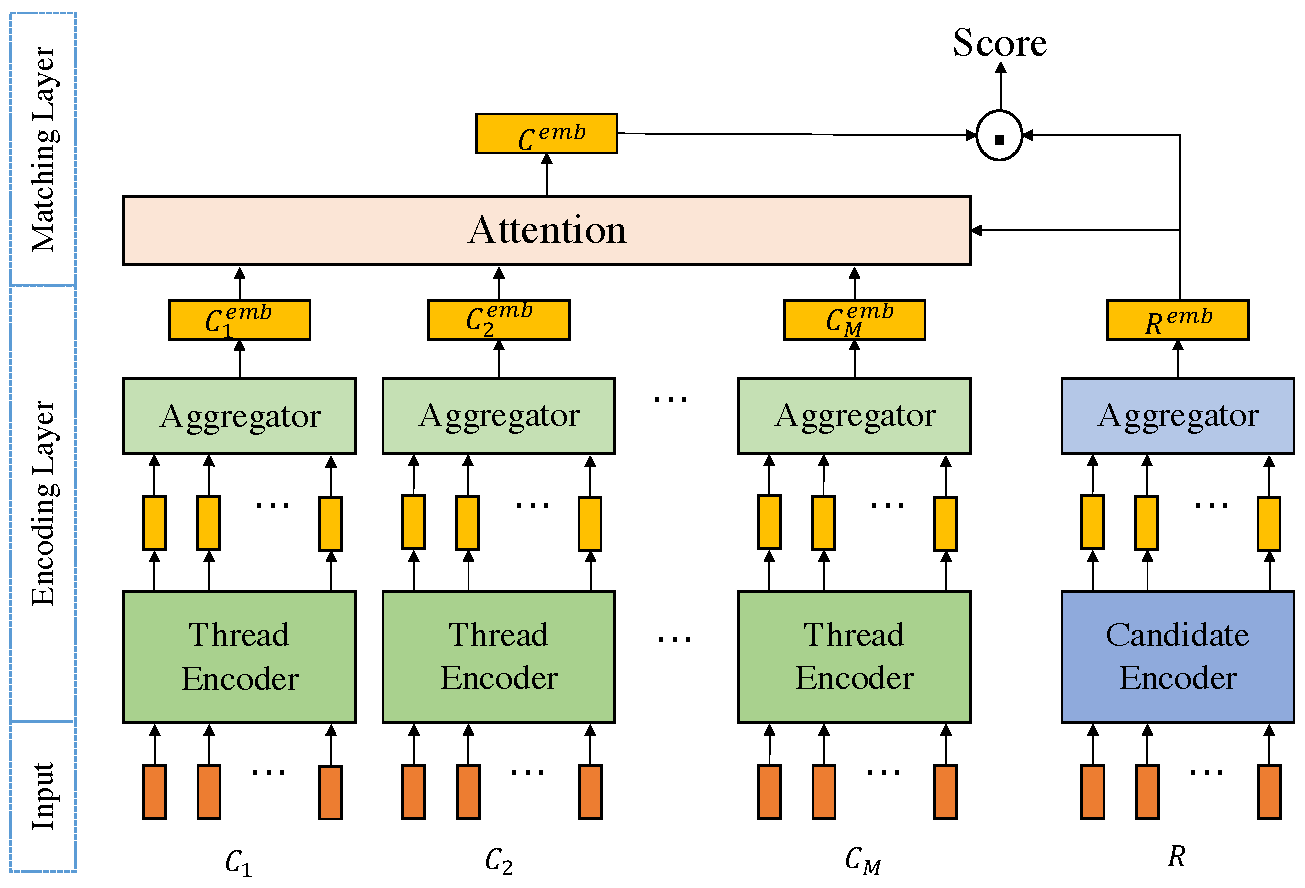
\includegraphics[scale=0.34]{pic/model-2.pdf}
	\caption{The architecture of Thread-Encoder model. All of the blocks in the same color share parameters.}
	\label{fig:model1}
\end{figure}

\subsubsection{Matching Layer}

Given the encoded threads $\langle C^{emb}_1, C^{emb}_2, ..., C^{emb}_M\rangle$ and candidate $R^{emb}$, we further use an attention layer to distill the information from the threads by attending the query $R^{emb}$ to each $C_m^{emb}$:

\begin{equation}
\begin{aligned}
C^{emb}&=\sum_{m=1}^Mw_mC^{emb}_m
\end{aligned}
\end{equation}
where

\begin{equation}
\begin{aligned}
s_m &= (R^{emb})^\top \cdot C^{emb}_m\\
w_m &= \exp(s_m)/\sum_{k=1}^M\exp(s_k)
\end{aligned}
\end{equation}

The final matching score is given by:
\begin{equation}
\begin{aligned}
S = F(C_1, C_2, ..., C_M, R) = (R^{emb})^\top\cdot C^{emb}
\end{aligned}
\label{eq:matching_score}
\end{equation}

We consider the other correct responses in a mini-batch as the negative candidates to accelerate the training process~\cite{MazareHRB18}. The whole model is trained to minimize the cross-entropy loss as follows:
\begin{equation}
\begin{aligned}
loss = - \frac{1}{A}\sum_{a=1}^{A}\sum_{b=1}^{A} L_{ab}\log(S_{ab})
\end{aligned}
\end{equation}
where $A$ is the batch size. $L_{ab}$ equals $1$ when $a=b$, otherwise $0$. $S_{ab}$ is the matching score in \eqnref{eq:matching_score}.

